\documentclass[russian,utf8,14pt,simple]{eskdtext}
\usepackage[numbertop, numbercenter]{eskdplain}

% - Полуторный интервал
\renewcommand{\baselinestretch}{1.50}
% - Отступ красной строки
\setlength{\parindent}{1.25cm}	
% - Шрифт Times New Roman
\renewcommand{\rmdefault}{ftm}

% - Наименование документа
\ESKDtitle{ }
% - Обозначение документа
\ESKDsignature{ФВС КР. Х.ХХХХХХХ 001 ПЗ}
% - Наименование предприятия
\ESKDcolumnIX{ТУСУР, ФВС, КИБЭВС-1208}
% - Проверил
\ESKDchecker{Давыдова Е.М.}	
% - Литера 
\ESKDletter{У}{}{}
% - Разработал
\ESKDauthor{КИБЭВС-1208}			

% - Убирает точку в списке литературы
\makeatletter
\def\@biblabel#1{#1 }

% - ГОСТ списка литературы
\bibliographystyle{gost2008}

% - Верикальные отступы заголовков 
\ESKDsectSkip{section}{1em}{1em}
\ESKDsectSkip{subsection}{1em}{1em}
\ESKDsectSkip{subsubsection}{1em}{1em}

% - Изменение заголовков
\usepackage{titlesec}
\titleformat{\section}{\centering\normalfont\normalsize}{\thesection}{1.0em}{}
\titleformat{\subsection}{\centering\normalfont\normalsize}{\thesubsection}{1.0em}{}
\titleformat{\subsubsection}{\centering\normalfont\normalsize}{\thesubsubsection}{1.0em}{}
\titleformat{\paragraph}{\normalsize}{\theparagraph}{1.0em}{}

% - Оставим место под ТЗ 
\setcounter{page}{4}

% - Для больших таблиц
\usepackage{longtable}
\usepackage{tabularx}
\renewcommand{\thetable}{\thesection.\arabic{table}}

% - Используем графику в документе
\usepackage{graphicx}
\graphicspath{{images/}}
\renewcommand{\thefigure}{\thesection.\arabic{figure}}

% - Для вставки гиперссылок
\usepackage[colorlinks]{hyperref}

% - Счётчики
\usepackage{eskdtotal}

% - Для переопределения списков
\makeatletter
\renewcommand{\theenumi}{\arabic{enumi}}
\renewcommand{\labelenumi}{\theenumi)}

\sloppy

\begin{document}

\newpage
\ESKDthisStyle{empty}

\begin{center}
Министерство образования и науки Российской Федерации\\
Федеральное государственное бюджетное образовательное учреждение высшего профессионального образования\\
ТОМСКИЙ ГОСУДАРСТВЕННЫЙ УНИВЕРСИТЕТ СИСТЕМ УПРАВЛЕНИЯ И РАДИОЭЛЕКТРОНИКИ (ТУСУР)\\
Кафедра комплексной информационной безопасности электронно-вычислительных систем (КИБЭВС)\\
\end{center}

\begin{tabbing}
XXXXXXXXXXXXXXXXXXXXXXXXXXX \=
XXXXXXXXXXXXXXXX\kill
\> УТВЕРЖДАЮ\\
\> заведующий каф.КИБЭВС\\
\> \underline{\ \ \ \ \ \ \ \ \ \ \ \ \ \ \ \ \ \ \ \ } А.А. Шелупанов\\
\> "\underline{\ \ \ \ \ }"\underline{\ \ \ \ \ \ \ \ \ \ \ \ \ \ \ \ \ \ \ \ } 2013г.\\
\end{tabbing}

\begin{center}
КОМПЬЮТЕРНАЯ ЭКСПЕРТИЗА\\
Отчет по групповому проектному обучению\\
Группа КИБЭВС-1208\\
\end{center}

\begin{tabbing}
XXXXXXXXXXXXXXXXXXXXXXXXXXX \=
XXXXXXXXXXXXXXXX\kill
\> Ответственный исполнитель\\
\> Студент гр. 520-1\\
\> \underline{\ \ \ \ \ \ \ \ \ \ \ \ \ \ \ \ \ \ \ \ } Никифоров Д. С.\\
\> "\underline{\ \ \ \ \ }"\underline{\ \ \ \ \ \ \ \ \ \ \ \ \ \ \ \ \ \ \ \ } 2014г.\\
\ \\
\> Научный руководитель\\
\> Аспирант каф.КИБЭВС\\
\> \underline{\ \ \ \ \ \ \ \ \ \ \ \ \ \ \ \ \ \ \ \ } Гуляев А. И.\\
\> "\underline{\ \ \ \ \ }"\underline{\ \ \ \ \ \ \ \ \ \ \ \ \ \ \ \ \ \ \ \ } 2014г.\\
\end{tabbing}
\vfill
\begin{center}
Томск -- 2014
\end{center}

\newpage
\ESKDthisStyle{empty}
\paragraph{\hfill РЕФЕРАТ \hfill}
Курсовая работа содержит \ESKDtotal{page} страниц, \ESKDtotal{figure} рисунков, \ESKDtotal{table} таблицы, \ESKDtotal{bibitem} источников, \ESKDtotal{appendix} приложение.

КОМПЬЮТЕРНАЯ ЭКСПЕРТИЗА, ФОРЕНЗИКА, ЛОГИ, QT, XML, GIT, LATEX, ЖУРНАЛЬНЫЕ ФАЙЛЫ, SKYPE, PIDGIN, WINDOWS, СЕРТИФИКАЦИЯ, РЕПОЗИТОРИЙ, XSLT, LIB, БИБЛИОТЕКИ.

Цель работы --- создание программного комплекса, предназначенного для проведения компьютерной экспертизы.

Задачей, поставленной на данный семестр, стало написание программного комплекса, имеющего следующие возможности: 
\begin{enumerate}
\item сбор и анализ событий системных журналов операционной системы;
\item сбор и анализ информации из журналов истории браузеров;
\item сбор и анализ истории переписки мессенджеров;
\item сбор и анализ событий журнальных файлов приложений;
\item поиск файлов по имени.
\end{enumerate}
В числе результатов работы данного семестра можно выделить следующие нововведения:

\begin{itemize}
\item использование в разработке системы контроля версий GIT;
\item разработка архитектуры проекта;
\item написание комплекса на C++ посредством кроссплатформенного инструментария разработки ПО Qt;
\item анализ дальнейших перспектив использования данного комплекса, в том числе перспективы внедрения данного комплекса в гос. структуры, занимающиеся информационной безопасностью;
\item использование системы компьютерной вёрстки TeX для написания документации.
\end{itemize}


Пояснительная записка выполнена в текстовом редакторе Vim.

\newpage
\ESKDthisStyle{empty}
\paragraph{\hfill Список исполнителей \hfill}
Моргуненко А.В. -- документатор.

Никифоров Д.С. -- программист, ответственный исполнитель, ответственный за написание части системы, работающей с логами системы.

Поляков И.Ю. -- программист, ответственный за написание части системы, работающей с логами мессенджеров.

Пономарёв А.К. -- аналитик.

\newpage
\ESKDstyle{plain}
\renewcommand\contentsname{\hfill Содержание \hfill}
\tableofcontents

\newpage
\ESKDstyle{plain}
\section{Введение}
Компьютерно-техническая экспертиза является классом инженерно-\\технических экспертиз, проводимых в целях поиска криминалистически значимой информации на носителях, её всестороннего исследование, и, как следствие, получения доказательственной информации и установления фактов, имеющих значение для уголовных, гражданских и административных дел, сопряжённых с использованием компьютерных технологий. Для проведения компьютерных экспертиз необходима высокая квалификация экспертов, так как при изучении представленных носителей информации, попытке к ним доступа и сбора информации возможно внесение в информационную среду изменений или полная утрата важных данных.

Компьютерная экспертиза, в отличие от компьютерно-технической экспертизы, затрагивает только информационную составляющую, в то время как аппаратная часть и её связь с программной средой не рассматривается.

На протяжении предыдущих семестров нами были рассмотрены такие направления компьютерной экспертизы, как исследование файловых систем, сетевых протоколов, организация работы серверных систем, механизм журналирования событий. Также нами были изучены основные задачи, которые ставятся перед сотрудниками правоохранительных органов, которые проводят компьютерную экспертизу, и набор чуществующих утилит, способных помочь эксперту в проведении компьютерной экспертизы. Было выявлено, что существует множество разрозненных программ, предназначенных для просмотра лог-файлов системы и таких приложений, как мессенджеры и браузеры, но для каждого вида лог-файлов необходимо искать отдельную программу. Так как ни одна из них не позволяет эксперту собрать воедино и просмотреть все логи системы, браузеров и мессенджеров, было решено создать для этой цели собственный автоматизированный комплекс, которому на данный момент нет аналогов.


\section{Назначение и область применения}
Разрабатываемый комплекс предназначен для автоматизации процесса сбора информации с исследуемого образа жёсткого диска.
\section{Постановка задачи}
\setcounter{figure}{0}
На данный семестр были поставлены следующие задачи:

\begin{itemize}
\item изучение архитектуры проекта <<Компьютерная экспертиза>> новыми участниками проектной группы;
\item изучение теоретического материала и основных инструментов разработки;
\item определение индивидуальных задач для каждого участника проектной группы;
\item исследование предметных областей в рамках индивидуальных задач; 
\item реализация новых программных модулей и доработка уже существующих;
\item изучение инструментов для генерации документации к программному коду проекта.
\end{itemize}

Задачи по проектированию модулей:

\begin{enumerate}
\item сбор и анализ информации из реестра Windows;
\item сбор и анализ информации из браузера Google Chrome;
\item сбор и анализ информации из почтового клиента Mozilla Thunderbird;
\item сбор и анализ информации из почтового клиента MS Outlook;
\item поиск медиа-файлов (аудио, видео, изображение) и извлечение мета-данных из них;
\item сбор информации об установленном ПО по остаточным файлам.
\end{enumerate}

\section{Инструменты}
\setcounter{figure}{0}
\subsection{Система контроля версий Git}
Для разработки программного комплекса для проведения компьютерной экспертизы было решено использовать Git.

Git --- распределённая система управления версиями файлов. Проект был создан Линусом Торвальдсом для управления разработкой ядра Linux  как противоположность  системе управления версиями Subversion (также известная как «SVN»). \cite{progit}

При работе над одним проектом команде разработчикоа необходим инструмент для совместного написания, бэкапирования и тестирования программного обеспечения. Используя Git, мы имеем:
\begin{itemize}
\item возможность удаленной работы с исходными кодами;
\item возможность создавать свои ветки, не мешая при этом другим разработчикам;
\item доступ к последним изменениям в коде, т.к. все исходники хранятся на сервере git.keva.su;
\item исходные коды защищены, доступ к ним можно получить лишь имея RSA-ключ;
\item возможность откатиться к любой стабильной стадии проекта.
\end{itemize}

Основные постулаты работы с кодом в системе Git:

\begin{itemize}
\item каждая задача решается в своей ветке;
\item необходимо делать коммит как только был получен осмысленный результат;
\item ветка master мержится не разработчиком, а вторым человеком, который производит вычитку и тестирование изменения;
\item все коммиты должны быть осмысленно подписаны/прокомментированы.
\end{itemize}


\subsection{Система компьютерной вёрстки \TeX}
\TeX\ --- это созданная американским математиком и программистом Дональдом Кнутом система для вёрстки текстов. Сам по себе \TeX\ представляет собой специализированный язык программирования.Каждая издательская система представляет собой пакет макроопределений этого языка.

\LaTeX\ --- это созданная Лэсли Лэмпортом издательская система на базе \TeX'а \cite{lvovskyi} \LaTeX\ позволяет пользователю сконцентрировать свои услия на содержании и структуре текста, не заботясь о деталях его оформления.

Для подготовки отчётной и иной документации нами был выбран \LaTeX\, так как совместно с системой контроля версий Git он предоставляет возможность совместного создания и редактирования документов. Огромным достоинством системы \LaTeX\ то, что создаваемые с её помощью файлы обладают высокой степенью переносимости. \cite{latexrus}

Совместно с \LaTeX\ часто используется Bib\TeX\ --- программное обеспечение для создания форматированных списков библиографии. Оно входит в состав дистрибутива \LaTeX\ и позволяет создавать удобную, универсальную и долговечную библиографию. Bib\TeX\ стал одной из причин, по которой нами был выбран \LaTeX\ для создания документации.

\subsection{Qt - кроссплатформенный инструментарий разработки ПО}
Qt --- это кроссплатформенная библиотека C++ классов для создания графических пользовательских интерфейсов (GUI) от фирмы Digia. Эта библиотека полностью объектно-ориентированная, что обеспечивает легкое расширение возможностей и создание новых компонентов. Ко всему прочему, она поддерживает огромнейшее количество платформ.

Qt позволяет запускать написанное с его помощью ПО в большинстве современных операционных систем путём простой компиляции программы для каждой ОС без изменения исходного кода. Включает в себя все основные классы, которые могут потребоваться при разработке прикладного программного обеспечения, начиная от элементов графического интерфейса и заканчивая классами для работы с сетью, базами данных и XML. Qt является полностью объектно-ориентированным, легко расширяемым и поддерживающим технику компонентного программирования.

Список использованных классов фраемворка QT
\begin{itemize}
\item iostream
\item QChar
\item QCryptographicHash
\item QDateTime
\item QDir
\item QDirIterator
\item QFile
\item QFileInfo
\item QIODevice
\item QList
\item QRegExp
\item QString
\item QTextStream
\item QtSql/QSqlDatabase
\item QVector
\item QMap
\item QXmlStreamReader
\item QXmlStreamWriter
\item Conversations
\end{itemize}

Класс QXmlStreamWriter представляет собой XML писателя с простым потоковым.

Класс QXmlStreamReader представляет собой быстрый синтаксически корректный XML анализатор с простым потоковым API. 

QVector представляет собой класс для создания динамических массивов.

Модуль QtSql/QSqlDatabase помогает обеспечить однородную интеграцию БД в ваши Qt приложения.

Класс QTextStream предоставляет удобный интерфейс для чтения и записи текста.

QTextStream может взаимодействовать с QIODevice, QByteArray или QString. Используя потоковые операторы QTextStream, вы можете легко читать и записывать слова, строки и числа. При формировании текста QTextStream поддерживает параметры форматирования для заполнения и выравнивания полей и форматирования чисел. \cite{qtdoc}

Класс QString предоставляет строку символов Unicode.

Класс QMap --- контейнерный класс для хранения элементов различных типов данных.

Класс QDateTime используется для работы с форматом даты, в который записывается информация о файле.

QString хранит строку 16-битных QChar, где каждому QChar соответствует один символ Unicode 4.0. (Символы Unicode со значениями кодов больше 65535 хранятся с использованием суррогатных пар, т.е. двух последовательных QChar.)

Unicode - это международный стандарт, который поддерживает большинство использующихся сегодня систем письменности. Это расширение US-ASCII (ANSI X3.4-1986) и Latin-1 (ISO 8859-1), где все символы US-ASCII/Latin-1 доступны на позициях с тем же кодом.

Внутри QString использует неявное совместное использование данных (копирование-при-записи), чтобы уменьшить использование памяти и избежать ненужного копирования данных. Это также позволяет снизить накладные расходы, свойственные хранению 16-битных символов вместо 8-битных.

В дополнение к QString Qt также предоставляет класс QByteArray для хранения сырых байт и традиционных нультерминальных строк. В большинстве случаев QString - необходимый для использования класс. Он используется во всем API Qt, а поддержка Unicode гарантирует, что ваши приложения можно будет легко перевести на другой язык, если в какой-то момент вы захотите увеличить их рынок распространения. Два основных случая, когда уместно использование QByteArray: когда вам необходимо хранить сырые двоичные данные и когда критично использование памяти (например, в Qt для встраиваемых Linux-систем). \cite{qtcross}

Класс QRegExp предоставляет сопоставление с образцом при помощи регулярных выражений.

Регулярное выражение, или ''regexp'', представляет собой образец для поиска соответствующей подстроки в тексте. Это полезно во многих ситуациях, например:

Проверка правильности -- регулярное выражение может проверить, соответствует ли подстрока каким-либо критериям, например, целое ли она число или не содержит ли пробелов.
Поиск -- регулярное выражение предоставляет более мощные шаблоны, чем простое соответствие строки, например, соответствие одному из слов mail, letter или correspondence, но не словам email, mailman, mailer, letterbox и т.д.
Поиск и замена -- регулярное выражение может заменить все вхождения подстроки другой подстрокой, например, заменить все вхождения \& на \&amp;, исключая случаи, когда за \& уже следует amp;.
Разделение строки -- регулярное выражение может быть использовано для определения того, где строка должна быть разделена на части, например, разделяя строку по символам табуляции.

QFileInfo  - Во время поиска возвращает полную информацию о файле.

Класс QDir обеспечивает доступ к структуре каталогов и их содержимого.

QIODevice представляет собой базовый класс всех устройств ввода/вывода в Qt.

Класс QCryptographicHash предоставляет способ генерации криптографических хэшей.
QCryptographicHash могут быть использованы для генерации криптографических хэшей двоичных или текстовых данных.В настоящее время MD4, MD5, и SHA-1 поддерживаются. \cite{qtcross}

QChar обеспечивает поддержку 16-битных символов Unicode.

\subsubsection{Aвтоматизация поиска журнальных файлов}

Для сканирования образа на наличие интересующих лог файлов использовался класс QDirIterator. После вызова происходит поочередный обход по каждому файлу в директории и поддиректории. Проверка полученного полного пути к файлу осуществляется регулярным выражением, если условие выполняется, происходит добавление в список обрабатываемых файлов.

\subsubsection{Реализация сохранения результатов работы программного комплекса в XML}

Cохранение полученных данных происходит в ранее выбранный формат XML(Extensible Markup Language). Для этого используется класс QXmlStreamReader и QxmlStreamWriter.
Класс QXmlStreamWriter представляет XML писателя с простым потоковым API.

QXmlStreamWriter работает в связке с QXmlStreamReader для записи XML. Как и связанный класс, он работает с QIODevice, определённым с помощью setDevice().

Сохранение данных реализованно в классе WriteMessage. В методе WriteMessages, структура которого представлена на UML диаграмме в разделе Архитектура.


\section{Технические характеристики}
\section {Технические характеристики}

%я не уверен, но помоему этот раздел надо бы подругому назвать =) 

\subsection {Постановка задачи}

На данный семестр были поставлены следующие задаи:

\begin{enumerate}
\item Определиться при помощи каких средств вести разработку
\item Разработать архитектуру проекта
\item Реализовать структуру проекта 
\item Определиться с форматом выходных данных
\item Реализовать несколько модулей
\end{enumerate}

\subsection {Выбор единого формата выходных файлов}

Для вывода результата был выбран формат XML-документов, так как с данным форматом лего работать при помощи программ, а результат работы данного комплекса в дальнейшем планируется обрабатывать при помощи программ

%и вот тут вброс про XML можно.

\subsubsubsubsection {Требования к аппаратному обеспечению}

Минимальные системные требования:\\
- Процессор 1ГГц Pentium 4;\\
- память 512 Мб;\\
- диск 9 Гб.

\subsubsubsubsection {Требования к программному обеспечению обеспечению}

На компьютерне должна быть установлена операционная система ubuntu 12.04 или выше, данная система должна иметь набор библиотек QT.
\subsection{Выбор единого формата выходных файлов}
Для вывода результата был выбран формат XML-документов, так как с данным форматом лего работать при помощи программ, а результат работы данного комплекса в дальнейшем планируется обрабатывать при помощи программ.

XML - eXtensible Markup Language или расширяемый язык разметки. Язык XML представляет собой простой и гибкий текстовый формат, подходящий в качестве основы для создания новых языков разметки, которые могут использоваться в публикации документов и обмене данными \cite{xml}. Задумка языка в том, что он позволяет дополнять данные метаданными, которые разделяют документ на объекты с атрибутами. Это позволяет упростить программную обработку документов, так как структурирует информацию.

Простейший XML-документ может выглядеть так:


\begin{verbatim}
<?xml version="1.0"?>
<list_of_items>
<item id="1"\><first/>Первый</item\>
<item id="2"\>Второй <subsub_item\>подпункт 1</subsub_item\></item\>
<item id="3"\>Третий</item\>
<item id="4"\><last/\>Последний</item\>
</list_of_items>
\end{verbatim}


Первая строка - это объявление начала XML-документа, дальше идут элементы документа <list\_of\_items> - тег описывающий начало элемента \\list\_of\_items, </list\_of\_items> - тег конца элемента. Между этими тегами заключается описание элемента, которое может содержать текстовую информацию или другие элементы (как в нашем примере). Внутри тега начала элемента так же могут указывать атрибуты элемента, как например атрибут id элемента item, атрибуту должно быть присвоено определенное значение.


\section{Разработка программного обеспечения}
\setcounter{figure}{0}

\subsection{Архитектура}
\subsection{Основной алгоритм}
В ходе разарботки был применен видоизменнённый шаблон проектирования Factory method.

%Описание шаблона и его модификации
Данный шаблон относится к классу порождающих шаблонов. Шаблоны данного класса - это шаблоны проектирования, которые абстрагируют процесс инстанцирования (создания экземпляра класса). Они позволяют сделать систему независимой от способа создания, композиции и представления объектов. Шаблон, порождающий классы, использует наследование, чтобы изменять инстанцируемый класс, а шаблон, порождающий объекты, делегирует инстанцирование другому объекту.
Основной алгоритм представлен на рисунке \ref{architech:architech}.

\begin{figure}[h!]
\center{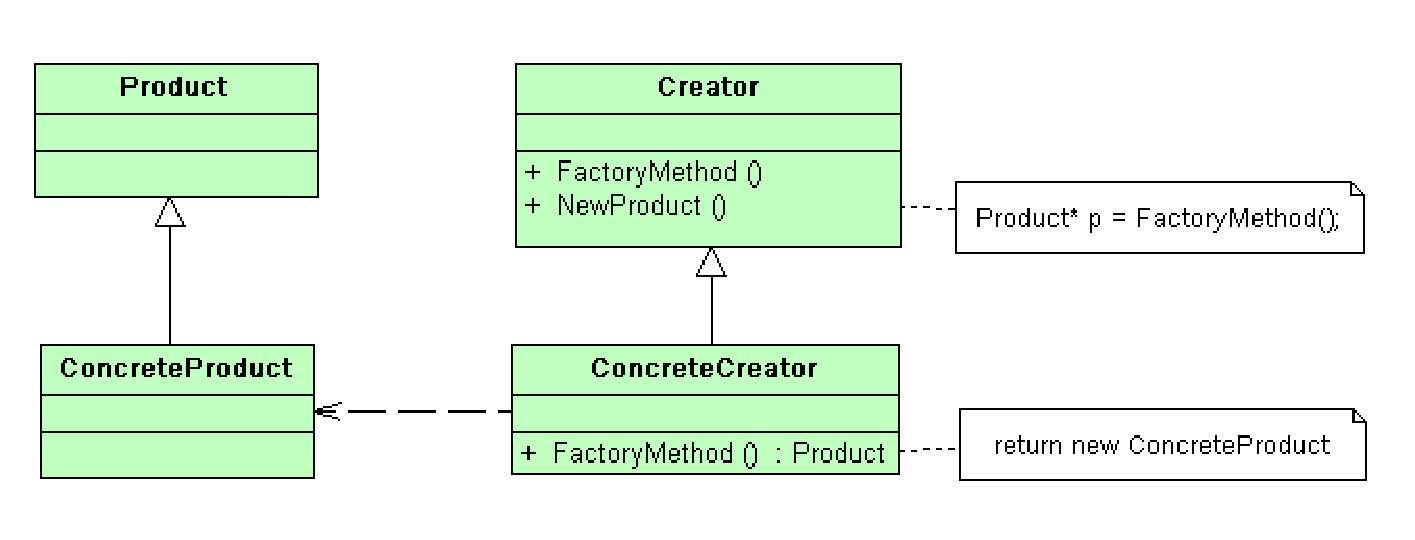
\includegraphics[width=0.9\linewidth]{architech}}
\caption{Основной алгоритм}
\label{architech:architech}
\end{figure}

Использование данного шаблона позволило нам разбить наш проект на независимые модули, что весьма упростило задачу разработки, так как написание алгоритма для конкретного таска не влияло на остальную часть проекта. При разработке был реализован базовый класс для работы с образом диска. Данный клас предназначался для формирования списка настроек, определения операционной системы на смонтированном образе и инстанционировании и накапливание всех необходимых классов-тасков в очереди тасков. После чего каждый таск из очереди отправлялся на выполнение. Блоксхема работы алгоритма (тут картинка alg_main.eps)

Каждый класс-таск порождался путем наследования от базового абстрактного класса который имеет 8 методов и 3 атрибута:

\begin{enumerate}
\item QString manual() - возвращает справку о входных параметрах данного таска;
\item void setOption(QStringList list) - установка флагов для поданных на вход параметров;
\item QString command() - возвращает команду для инициализации такска вручную;
\item bool supportOS(const coex::typeOS \&os) - возвращает флаг, указывающий на возможность использования данного таска для конкретной операционной системы;
\item QString name() - возвращает имя данного таска;
\item QString description() - возвращает краткое описание таска;
\item bool test() - предназначена для теста на доступность таска;
\item bool execute(const coex::config \&config) - запуск таска на выполнение;
\item QString m\_strName - хранит имя таска;
\item QString m\_strDescription - хранит описание таска;
\item bool m\_bDebug - флаг для параметра --debug;
\end{enumerate}

На данный момент в проекте используется восемь классов. UML-диаграмма классов представлена на рисунке (тут картинка UML.eps)

Классы taskSearchSyslogsWin, taskSearchPidginWin и taskSearchSkypeWin - наследники от класса task являются тасками. Класс winEventLog и _EVENTLOGRECORD предназначины для конвертации журнальных файлов операционной системы Windows XP, а класс writerMessages для преобразования истории переписки.
\subsection{Сбор и анализ системных журналов Windows (III семестр)} % - Отчёт Димы
Анализ журналов операционных систем может помочь при решении многих задач. Примером таких задач может быть попытка восстановления системы после поломок, поиск причин неполадок системы, просмотр журналов с целью выявления активности приложений в определенные периоды и т.д. и т.п. Также, анализ журнальных файлов является неотъемлемой частью компьютерно-технических экспертиз.

При исследовании компьютеров задача анализа журнальных файлов ставится на этапе «выявление и изучение его роли в рассматриваемом деле», так как именно в журнальных файлах операционной системы хранится информация о действиях производимых на данном компьютере.

Для проведения компьютерных экспертиз существует множество специализированных программных средств, как платных так и свободно распространяемых. Примером такого средства является «OSForensics». Данный инструмент позволяет проводить множество различных исследований таких как просмотр содержимого оперативной памяти, поиск подозрительных файлов на жестком диске, составления списка программ установленных на исследуемом компьютере. Но бесплатная версия не предоставляет никаких средств по работе с журналами операционной системы. Данный факт подтолкнул к созданию собственного программного средства для проведения компьютерных экспертиз.

В данной работе описывается работа по созданию модуля для данного программного средства, позволяющего в автоматическом режиме находить, читать и конвертировать журнальные файлы операционной системы Windows XP в XML-документы, понятные для человека и легко обрабатываемые при помощи\\ электронно-вычислительных средств.

\subsubsection{Общие сведения о журнальных файлах}

В операционной системе Windows XP по умолчанию есть четыре журнала:

\begin{enumerate}
\item Журнал приложений
\item Журнал безопасности
\item Журнал установки
\item Журнал системы
\end{enumerate}

Каждый из этих журналов содержит определенный тип информации. Журналы приложений содержат информацию о запуске и остановке процессов приложений, изменении статуса каждого приложения, а также предупреждения и ошибки связанные с приложениями.

Журнал безопасности содержит информацию о входах в систему, и события связанные с безопасностью системы, например превышение количества попыток неправильно введенных подряд паролей.

Журнал установки содержит информацию об установке и обновлении компонентов системы.

Журнал системы хранит информацию о системных событиях. Например изменение схемы энергопотребления или различного рода предупреждения и ошибок.

Каждый журнал хранится в соответствующем файле с расширением .evt. Эти файлы хранятся в папке \%windows\%/system32/config. Эти файлы имеют специальную структуру.

\subsubsection{Структура журнальных файлов операционной системы Windows XP}

Все журнальные файлы операционной системы Windows XP имеют единую структуру. Файл представляет собой последовательность записей бинарных данных. Каждая запись – это структура имеющая семнадцать полей \cite{evt}.

Первые 4 байта содержат длину события в байтах, после длинны идет 4 байтный системный код сообщения. Затем 4 байтовый номер записи, после него дата создания записи, время создания, идентификатор события, тип события и так далее. Ниже приведен список полей записи, предназначенной для считывания одного события из журнального файла.

\begin{itemize}
\item uint32 Length; 
\item uint32 Reserved;
\item uint32 RecordNumber;
\item uint32 TimeGenerated;
\item uint32 TimeWritten;
\item uint32 EventID;
\item uint16 EventType;
\item uint16 NumStrings;
\item uint16 EventCategory;
\item uint16 ReservedFlags;
\item uint32 ClosingRecordNumber;
\item uint32 StringOffset;
\item uint32 UserSidLength;
\item uint32 UserSidOffset;
\item uint32 DataLength;
\item uint32 DataOffset;
\item byte[] Data.
\end{itemize}

Из сторонних источников \cite{evt} стало известно о пяти типах событий (поле EventType) (значение - тип события):

\begin{enumerate}
\item 0x0001 - Error event;
\item 0x0010 – Failure Audit event;
\item 0x0008 - Success Audit event;
\item 0x0004 - Information event;
\item 0x0002 - Warning event.
\end{enumerate}

У поля EventID удалось определить четыре значения:

\begin{enumerate}
\item 0x00 – Success;
\item 0x01 – Informational;
\item 0x02 – Warning;
\item 0x03 – Error.
\end{enumerate}

Среди множества полей записи события были выделены поля содержащие информацию о типе события, времени возникновения события и создания записи, пользователя от имени которого была сделана запись, а также поле Data - поле с бинарными данными, в которых записана подробная информация о событии.

\subsubsection{Алгоритм работы модуля}

Модуль выполняет две задачи: поиск журнальных файлов на образе диска и конвертацию каждого файла в XML-документ. Первая задача выполняется при помощи библиотек QDir и QDirIterator из Qt Framework.

QDir — библиотека позволяющая работать с конкретной директорией. Создав объект данного типа с указанием директории мы получим доступ к этой директории в программе и сможем работать в ней (просматривать содержимое; удалять, создавать или копировать файлы; создавать поддиректории). Данный объект так же поддерживать разные наборы фильтров выходных данных которые могут отсеивать ненужную информацию.

QDirIterator — библиотека, предназначенная для работы с файловой системой начиная с определенной директории как точки входа. Создав объект данного типа с указанием директории мы получим все пути которые существуют в файловой системе и начинаются с указанной директории. Данный объект поддерживает фильтрацию которая помогает выделять только необходимую информацию, исключая то, что нас не интересует, например можно вывести список только тех файлов, которые находятся в данной директории или поддиректориях, или исключить вывод символьных ссылок. Объекты данного типа используются для поиска файлов или папок на образе исследуемого диска.

Так же данные библиотеки позволяют создавать объект QFile, который позволяет работать с файлом, путь к которому передается как параметр при создании, данный объект позволяет получить базовую информацию о файле, такую как относительный или абсолютный путь до этого файла, размер файла, тип файла или его имя. Так же позволяет перемещать или копировать данный файл. Поиск работает по алгоритму представленному на рисунке \ref{evtsearch:evtSearch}.

\begin{figure}[ht]
\center{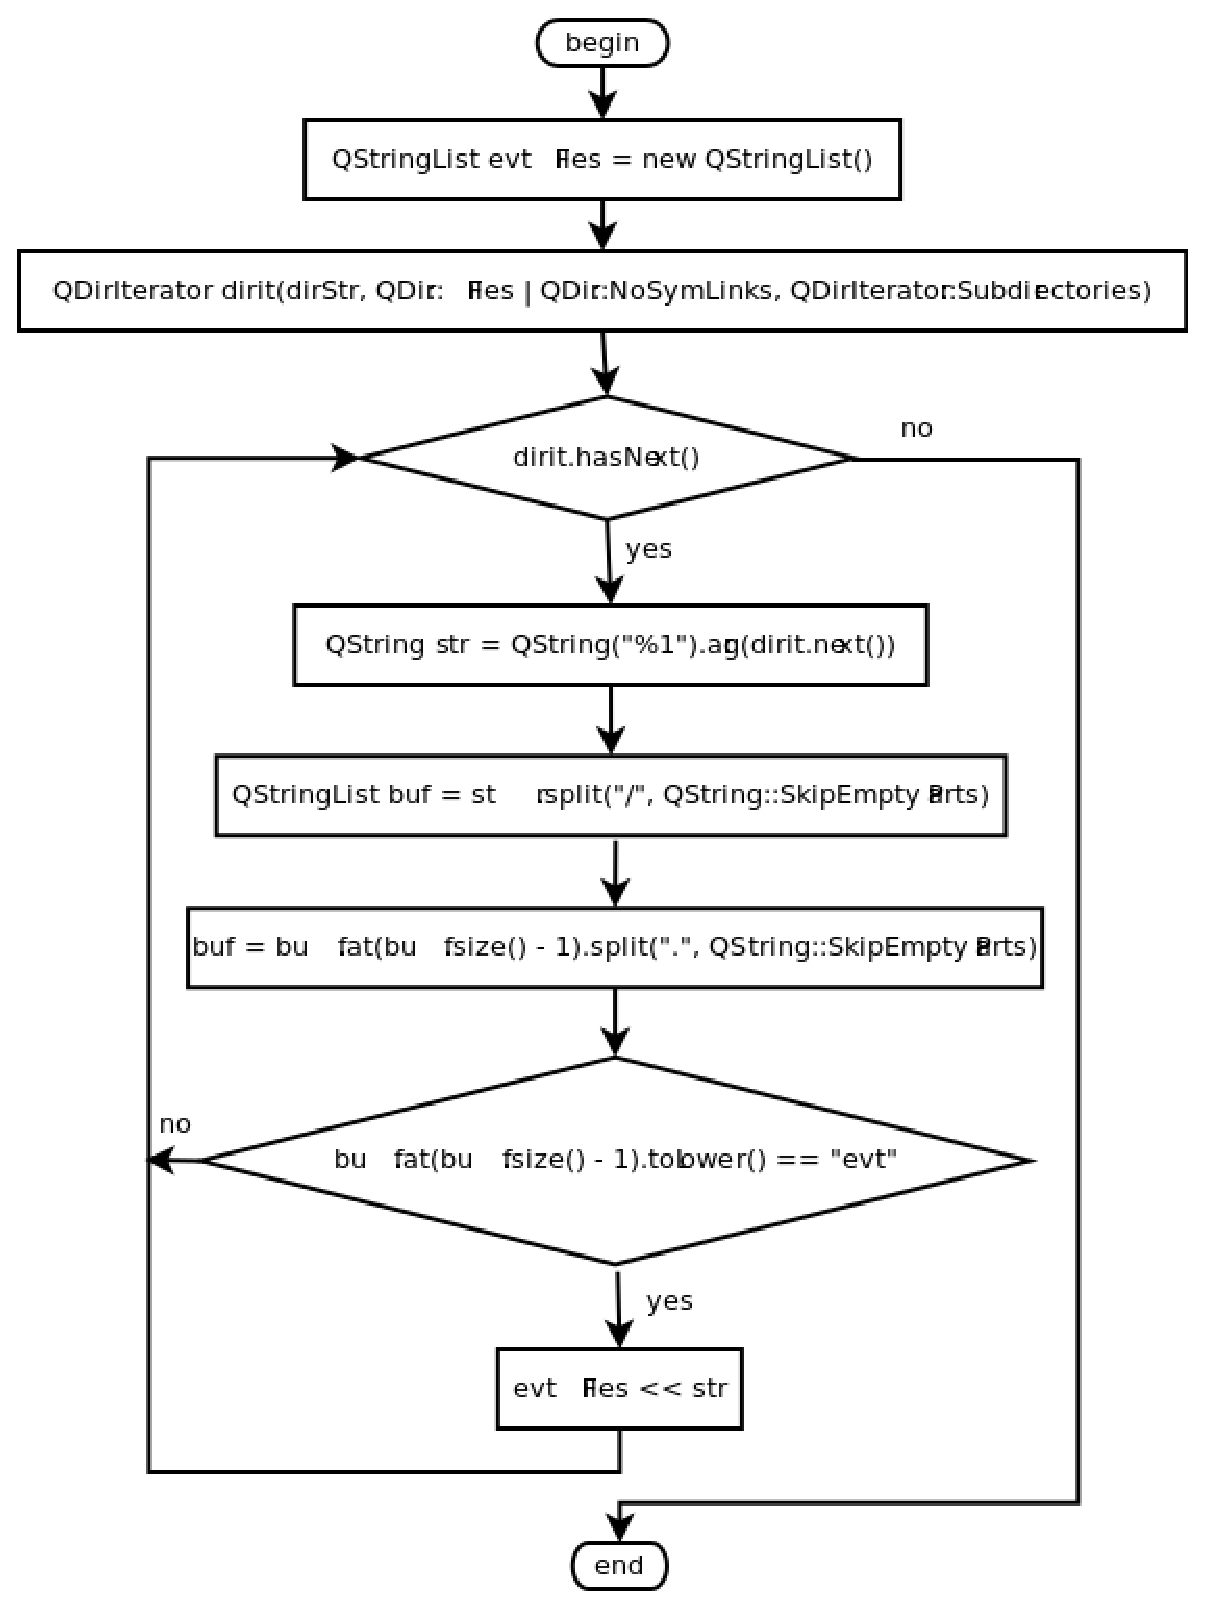
\includegraphics[width=0.6\linewidth]{evtSearch}}
\caption{Алгоритм поиска файлов с расширением *.evt}
\label{evtsearch:evtSearch}
\end{figure}

На выходе данного алгоритма мы получаем объект QStringList который содержит пути до всех найденных .evt файлов. Каждый экземпляр коллекции строк данного объекта передается в конструктор объекта winEventLog, который и конвертирует указанный файл в XML-документ. Алгоритм работы конвертора представлен на рисунке \ref{evtxml:evtToXML}.

\begin{figure}[ht]
\center{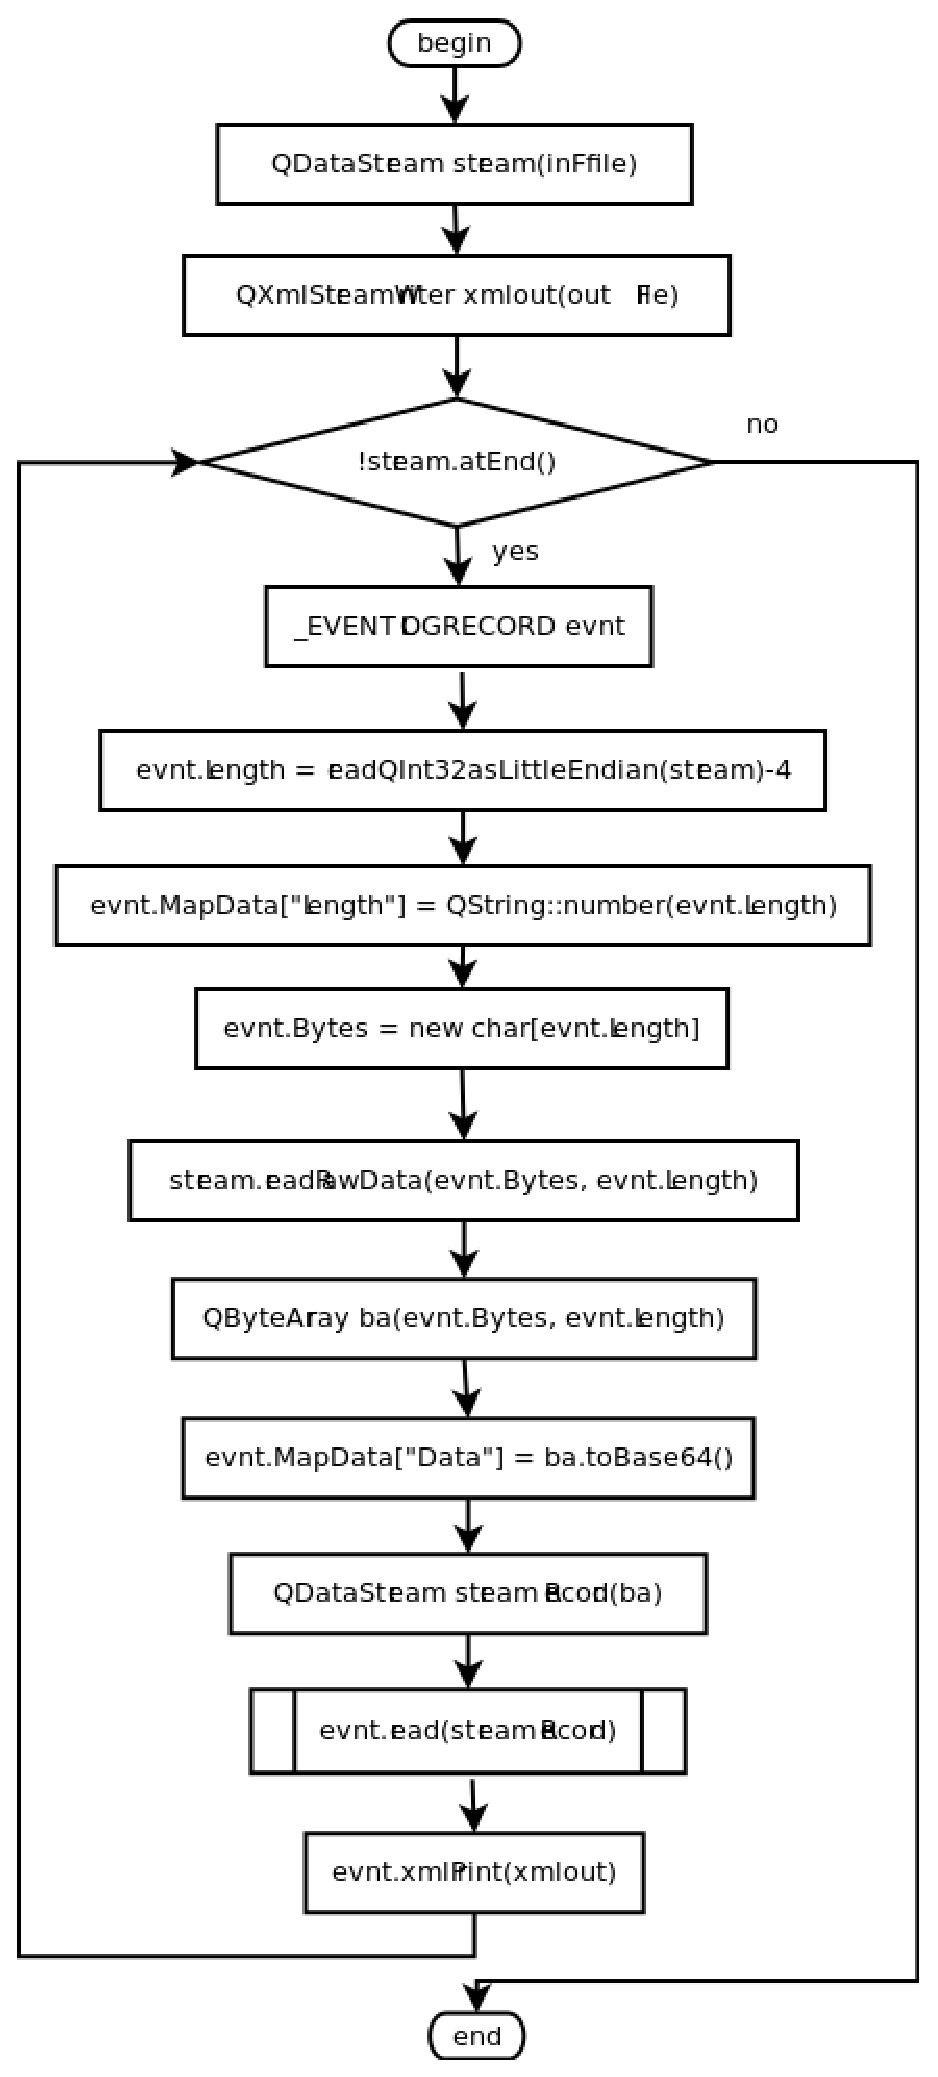
\includegraphics[width=0.4\linewidth]{evtToXML}}
\caption{Алгоритм конвертирования файлов *.evt в формат XML}
\label{evtxml:evtToXML}
\end{figure}

\subsection{Сбор и анализ системных журналов Windows (IV семестр)} 
\subsubsection{Введение}

Продолжая разработку данного программного продукта стало ясно что, несмотря на выбранный шаблон проектирования, добавление нового функционала осложняется тем, что при добавлении новой функции приходится пересобирать весь проект. Это неправльиный подход, так как не позволяет обновлять приложение. Для исправления этой ситуации необходимо доработать архитектуру приложения таким образом, что бы добавление новых функций не приводило к пересборке всего проекта. Это так же позволит проще обновлять проект в дальнейшем. 

После доработки архитектуры, необходимо будет переделать проект, переделать реализацию всего фукционала, а так же свести все ветки разработки в одну, так как на данный момент не все изменения применены к проекту. 

Сформулируем задачи на семестр:

\subsubsection{Задачи на семестр}

\begin{enumerate}
\item переработать архитектуру проекта для более легкого добавления новых функций
\item реализовать данную архитектуру
\item переделать готовые task'и для работы с текущей архитектурой
\item смерджить ветки разработки git
\end{enumerate}

\subsubsection{Новая архитектура}

С увеличением количества тасков возникла проблема с обновлением кода, так как используемый подход предполагал монолитную программу и все таски хоть и были стандартизированы при помощи шаблона разработки factory, всё равно являлись частью основной программы и для добавления тасков или их обновления необходимо постоянно перекомпилировать весь проект. Данная ситуация крайне неудобна при разработки и тестировании, поэтому необходимо было разделить проект на независимые модули.

В языке программирования C++ есть возможность создания библиотек. Библиотеки -- это бинарные файлы в которых хранится коллекции классов и функций. Эти классы и функции можно использовать в любой программе в которой данная библиотека подулючается. Подключать библиотеки в программу можно статически (на этапе компиляции программы) или динамически (непосредственно при выполнении программы). У нашего проекта есть <<скелет>> и таски, каждый из которых работает независимо друг от друга и обменивается данными только со скелетом. 

Так как каждая библиотека является самостоятельным файлом с исполняемым кодом, то для его создания и изменения необходим отдельный проект разработки, а значит если мы захотим изменить что-либо внутри библиотеки, то практически наверняка нам не нужно будет перекомпилировать весь проект. Это значительно упрощает операцию обновления программного комплекса. Было принято решение вынести реализацию всех функций скелета в отдельную статическую библиотеку. А все таски оформить в виде динамических библиотек. 

Данное решение повлекло за собой ряд проблем:
\begin{enumerate}
\item Необходимо разработать структуру динамических библотек для тасков программного комплекса;
\item Необходимо изменить механизм работы с тасками;
\item Необходимо изменить механизм разбора и передачи параметров в основной части программного комплекса;
\item Разработать механизм передачи информации в механизм разбора и передачи параметров.
\end{enumerate}

\subsubsection{библиотеки в С++ и их использование}

Библиотеки предоставляют программисту возможность использовать при разработке программы готовые фрагменты кода. В библиотеки могут быть включены подпрограммы, структуры данных, классы, макросы. В QT для создания библиотеки необходимо укахать в pro-файле проекта добавить строчку \\
TEMPLATE = lib\\
Данная строчка указывает компилятору на то, что мы компилируем библиотеку. После чего в файле исходного кода описывается всё необходимое и после компиляции мы получим файл библиотеки. Для создания динамической библиотеки необходимо добавить в pro-файл ещё строчку: \\
CONFIG += dll\\
А так же в заголовочном файле библиотеки поместить описание прототипов функций которые мы хотим подключать динамически в конструкцию\\
extern <<C>>{ <<описание прототипов>> }\\
Это необходимо для того, что бы при сборке библиотеки функции не поменяли имена. Если не добавить данную конструкцию, то компилятор при сборке изменит имена функций и обратиться к ним динамически не получится.

Для использования разработанной статической библиотеки необходимо просто указать в файле исходного кода строчку \\
\# include <<abolute/part/to/library/file>> \\
Либо поместить созданную библиотеку в папку с системными библиотеками (или добавить в настройки операционной системы путь до созданной библиотеки), тогда можно подключать библиотеку так же как и стандартные библиотеки (имя библиотеки в треугольных скобках)

Динамические библиотеки используются по-другому. Загрузка функции из динамической библиотеки происходит в три этапа: 

\begin{enumerate}
\item Загрузка библиотеки;
\item Описание шаблона для вызова функции:
\item Вызов функции.
\end{enumerate}

В качестве примера на рисунке \ref{ris:dinLib} представлен пример вызова функции foо, которая принимает на вход один аргумент типа int и возвращает его удвоенное значение. функция находится в библиотеке exampleLib. Загрузка библиотеки производится при помощи средств, предоставляемых Qt framework: 
%вот тут короче рисуночек dinLib из папки images

\begin{figure}[ht] 
\center{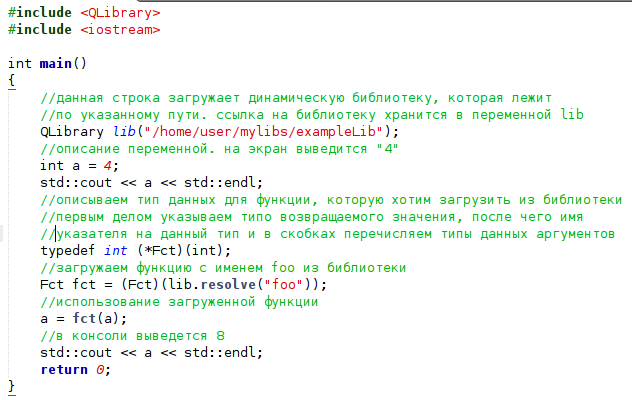
\includegraphics[width=1\linewidth]{dinLib}}
\caption{Пример вызова функции foo}
\label{ris:dinLib}
\end{figure}

\subsubsection{task = динамическая библиотека}

Для того, что бы программа могла работать с каждым таском, как с динамической библиотекой, необходимо что бы все библиотеки были созданы по одному шаблону. То есть в каждой библиотеке должен быть определенный набор функций с определенным именем и входными параметрами к которым можно обращаться при загрузки библиотеки. 

В каждой библиотеке необходимо определить две функции:

\begin{enumerate}
\item функция, возвращающая информацию о таске (имя таска и возможный набор параметров, предназначенных для данного таска)
\item функция выполнения данного таска, которая возвращает логическое значение по окончанию работы, на вход она принимает переменную со всеми настройками, введенными пользователем
\end{enumerate}

На данный момент механизм разбора флагов не был реализван. Структура библиотеки представлена на рисунке \ref{ris:exampleLib}.
%вот тут короче рисунок exampleLib из папки images

\begin{figure}[ht] 
\center{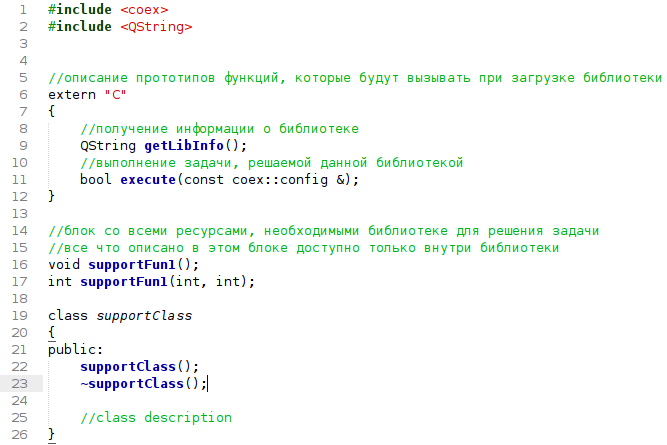
\includegraphics[width=1\linewidth]{exampleLib}}
\caption{Структура библиотеки}
\label{ris:exampleLib}
\end{figure}

Все реализованные таски были оформлены в виде динамических библиотек. Алгоритмы обработки данных изменению не подвергались.

\subsubsection{новый механизм работы с тасками}

Для того, что бы было возмодно добавлять в наш комплекс новые таски без перекомпиляции скелета комплекса мы оформили их в виде динамических библиотек, каждая из которых реализована по шаблону, рассмотренному выше. Все библиотеки, которые мы хотим загружать при работе программы мы помещаем в специальную дирректорию libs рядом с исполняемым файлом. При запуске программа просматривает данную дирректорию и поочередно загружает каждую библиотеку и запускает её на выполнение (если это возможно). 

Алгоритм работы данного механизма представлен на рисунке \ref{ris:initTasks}
%вот тут короче рисунок initTasks из папки images

\begin{figure}[ht] 
\center{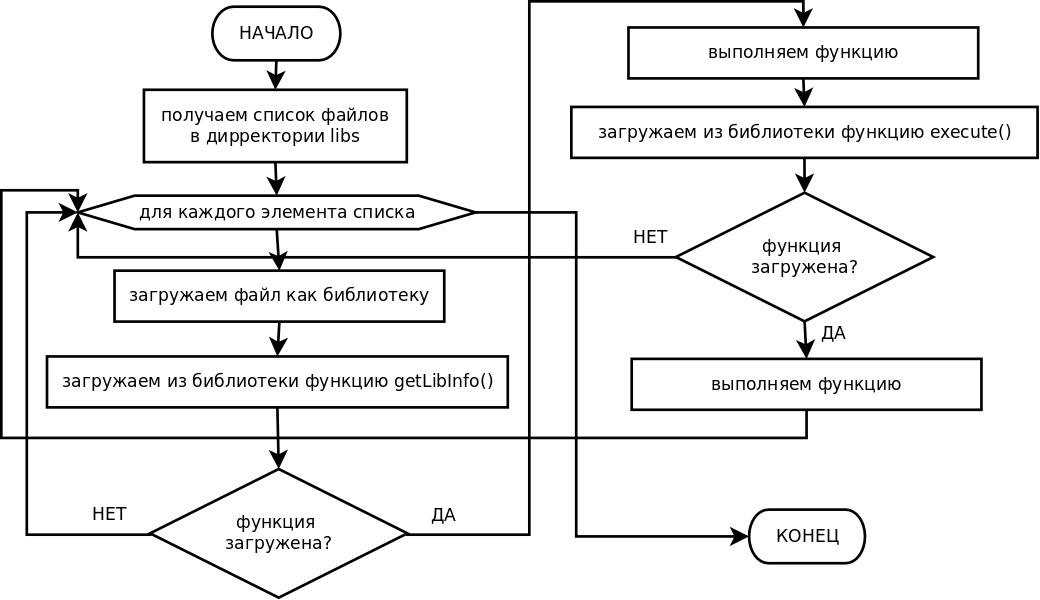
\includegraphics[width=1\linewidth]{initTasks}}
\caption{Пример вызова функции foo}
\label{ris:initTasks}
\end{figure}

\subsubsection{мерджим ветки git}

Разработка комплекса велась двумя разработчиками, каждый из которых работал в своей ветке разработки системы контроля версий git. Необходимо было собрать все изменнеия проекта воедино. Обычно для этого используются инструменты, предстовавляемые самим gitом, но так как в проекте была изменена архитектура (по сути был создан новый проект, который делали их частей старого), то было принято решение просто получить все изменнеия с каждой ветки для каждого проекта и оформить последнии версии тасков в виде динамических библиотек. Данный подход повзолил избежать процедуры разрешения конфликтов. На данный момент новая версия проекта находится в ветке master и содержит все последнии изменения предыдущего проекта. Разработка первой версии комплекса остановлена и, после того как весь код старого проекта будет использован, данная версия комплекса будет удалена.

\newpage
\subsection{Cбор и анализ истории переписки мессенджеров (III семестр)} % - Отчёт Игоря
\section{TaskSearchArchive}

\subsection{Структура RAR архива}
RAR — проприетарный формат сжатия данных и условно-бесплатная программа-архиватор. Имеет расширение .rar, .rev, .r00 или .r01

Определение архивного файла RAR
RAR-архив состоит из блоков переменной длины с заголовками по 7 байт каждый. Любой архив содержит как минимум два блока MARK_HEAD и MAIN_HEAD. Первый содержит информацию о том, что перед нами RAR, и выглядит как "0x 52 61 72 21 1A 07 00" в HEX'ах, или “0x 52 45 7E 5E” в старых версиях . Третий байт 0х72 как раз таки указывает на то, что это Marker Header. Слово 00 07 в little-endian содержит длину блока. Как раз таки 7 байт.[1]

Второй блок Main Header начинается сразу же после первого и должен содержать 13 байт и иметь маркировочный байт равным 0x73. После него в файле уже начинаются данные — будь-то сжатый файл (маркет 0х74 в третьем байте заголовка блока), комментарий к архиву, дополнительная информация или, к примеру, recovery-запись.[2]

Формат архивного файла RAR
                
Файл архива состоит из блоков разной длины.
В самом начале архива стоит блок-маркер, после которого идёт блок заголовка архива, за которым в произвольном порядке следуют блоки остальных типов.
                
                Каждый блок начинается со следующих полей:         
                 
HEAD_CRC 
2 байта 
CRC всего блока или его части
HEAD_TYPE 
1 байт
Тип блока 
HEAD_FLAGS
16 бит ( =2 байта) 
Флаги(*) блока     
HEAD_SIZE     
2 байта
Размер блока 
ADD_SIZE
4 байта 
Добавление к размеру блока (необязательное поле — может отсутствовать) 
            
Во всех блоках следующие биты в HEAD_FLAGS (*) имеют одинаковое значение:         
предпоследний 14-й (смещение 0х4000) — если = true (*), то старые версии RAR будут игнорировать этот блок и удалять его при изменении архива; иначе блок копируется в новый архивный файл при изменении архива;
последний 15-й (смещение 0х8000) — если = true, то поле ADD_SIZE присутствует в блоке, иначе — отсутствует.
                
Заявленные типы блоков (возможные значения HEAD_TYPE):             
            
0x72 (*) — блок-маркер;
0x73 — заголовок архива;
0x74 — заголовок файла;
0x75 — заголовок комментария старого типа;
0x76 — электронная подпись старого типа;
0x77 — субблок старого типа;
0x78 — информация для восстановления старого типа;
0x79 — электронная подпись старого типа;
0x7A — субблок.
            
Форматы блоков
Блок-маркер (MARK_HEAD)
HEAD_CRC = 0x6152;
HEAD_TYPE = 0x72;
HEAD_FLAGS = 0x1a21;
HEAD_SIZE = 0x0007;
            
Заголовок архива (MAIN_HEAD)
HEAD_CRC = CRC полей от HEAD_TYPE до RESERVED2;
HEAD_TYPE = 0x73;
HEAD_FLAGS ( =16 бит):                     

0-й бит (*) (смещение 0x0001 (*)) — Атрибут тома (том многотомного архива) (*)
1-й бит (смещение 0x0002) — Присутствует архивный комментарий (RAR 3.x использует отдельный блок комментария и не устанавливает этот флаг)
2-й бит (смещение 0x0004) — если = true, то архив заблокирован для изменений
3-й бит (смещение 0x0008) — если = true, то это — непрерывный (solid) архив
4-й бит (смещение 0x0010) — если = true, то используется новая схема именования томов ('volname.partN.rar'), иначе — старая ('volname.rN')
5-й бит (смещение 0x0020) — Присутствует информация об авторе или электронная подпись (AV) (RAR 3.x не устанавливает этот флаг)
6-й бит (смещение 0x0040) — Присутствует информация для восстановления
7-й бит (смещение 0x0080) — Заголовки блоков зашифрованы
8-й бит (смещение 0x0100) — Первый том (устанавливает только RAR 3.0 и выше)
Остальные биты (с 9 по 15-й) зарезервированы для внутреннего использования

HEAD_SIZE (*) = Общий размер архивного заголовка, включая архивные комментарии;
RESERVED1 (2 байта) - Зарезервировано;
RESERVED2 (4 байта) - Тоже зарезервировано;
    
\subsection{Структура ZIP архива}                
Инфо http://habrahabr.ru/post/100200/

ZIP файл состоит из трех областей:
сжатые/несжатые данные, (последовательность структур Local File Header, сами данные и необязательных Data descriptor)
центральный каталог (последовательность структур Central directory file header)
описание центрального каталога (End of central directory record)
С начала файла идет набор из Local File Header, непосредственно данные и (необязательно) структура Data descriptor. Затем структуры типа Central directory file header для каждого файла и папки в ZIP архиве и завершает все это структура End of central directory record.
Local File Header
Используется для описания метаданных файла (имя файла, контрольная сумма, время и дата модификации, сжатый/несжатый размер). Как правило сразу после этой структуры следует содержимое файла.
struct LocalFileHeader
{
    // Обязательная сигнатура, равна 0x04034b50
    uint32_t signature;
    // Минимальная версия для распаковки
    uint16_t versionToExtract;
    // Битовый флаг
    uint16_t generalPurposeBitFlag;
    // Метод сжатия (0 - без сжатия, 8 - deflate)
    uint16_t compressionMethod;
    // Время модификации файла
    uint16_t modificationTime;
    // Дата модификации файла
    uint16_t modificationDate;
    // Контрольная сумма
    uint32_t crc32;
    // Сжатый размер
    uint32_t compressedSize;
    // Несжатый размер
    uint32_t uncompressedSize;
    // Длина название файла
    uint16_t filenameLength;
    // Длина поля с дополнительными данными
    uint16_t extraFieldLength;
    // Название файла (размером filenameLength)
    uint8_t *filename;
    // Дополнительные данные (размером extraFieldLength)
    uint8_t *extraField;
};
Сразу после этой структуры идут данные размером compressedSize при использовании сжатия или размером uncompressedSize в противном случае.
Иногда бывает невозможно вычислить данные на момент записи LocalFileHeader, тогда в crc32, compressedSize и uncompressedSize записываются нули третий бит в generalPurposeBitFlag ставится в единицу и после LocalFileHeader добавляется структура типа Data descriptor.
Data descriptor
Если по какой-то причине содержимое файла невозможно создать одновременно с заголовком типа Local File Header, то сразу после него следует структура Data descriptor, где идет находится дополнение метаданных для Local File Header (контрольная сумма, сжатый/несжатый размер). Откровенно говоря, мне такие файлы не попадались, поэтому больше того, чем написано в википедии сказать не могу.
struct DataDescriptor
{
    // Необязательная сигнатура, равна 0x08074b50
    uint32_t signature;
    // Контрольная сумма
    uint32_t crc32;
    // Сжатый размер
    uint32_t compressedSize;
    // Несжатый размер
    uint32_t uncompressedSize;
};
Central directory file header
Расширенное описание метаданных файла. Содержит дополненную версию LocalFileHeader (добавляются поля номер диска, файловые атрибуты, смещение до Local File Header от начала ZIP файла).
struct CentralDirectoryFileHeader
{
    // Обязательная сигнатура, равна 0x02014b50 
    uint32_t signature;
    // Версия для создания
    uint16_t versionMadeBy;
    // Минимальная версия для распаковки
    uint16_t versionToExtract;
    // Битовый флаг
    uint16_t generalPurposeBitFlag;
    // Метод сжатия (0 - без сжатия, 8 - deflate)
    uint16_t compressionMethod;
    // Время модификации файла
    uint16_t modificationTime;
    // Дата модификации файла
    uint16_t modificationDate;
    // Контрольная сумма
    uint32_t crc32;
    // Сжатый размер
    uint32_t compressedSize;
    // Несжатый размер
    uint32_t uncompressedSize;
    // Длина название файла
    uint16_t filenameLength;
    // Длина поля с дополнительными данными
    uint16_t extraFieldLength;
    // Длина комментариев к файлу
    uint16_t fileCommentLength;
    // Номер диска
    uint16_t diskNumber;
    // Внутренние аттрибуты файла
    uint16_t internalFileAttributes;
    // Внешние аттрибуты файла
    uint32_t externalFileAttributes;
    // Смещение до структуры LocalFileHeader
    uint32_t localFileHeaderOffset;
    // Имя файла (длиной filenameLength)
    uint8_t *filename;
    // Дополнительные данные (длиной extraFieldLength)
    uint8_t *extraField;
    // Комментарий к файла (длиной fileCommentLength)
    uint8_t *fileComment;
};
End of central directory record (EOCD)
Эта структура записывается в конце файла. Содержит следующие поля: номер текущего диска, количество записей Central directory file header в текущем диске, общее количество записей Central directory file header.
struct EOCD
{
    // Обязательная сигнатура, равна 0x06054b50
    uint32_t signature;
    // Номер диска
    uint16_t diskNumber;
    // Номер диска, где находится начало Central Directory
    uint16_t startDiskNumber;
    // Количество записей в Central Directory в текущем диске
    uint16_t numberCentralDirectoryRecord;
    // Всего записей в Central Directory
    uint16_t totalCentralDirectoryRecord;
    // Размер Central Directory
    uint32_t sizeOfCentralDirectory;
    // Смещение Central Directory
    uint32_t centralDirectoryOffset;
    // Длина комментария
    uint16_t commentLength;
    // Комментарий (длиной commentLength)
    uint8_t *comment;
};
Папки в ZIP файле представлены двумя структурами Local File Header и Central directory file header с нулевым размером и контрольной суммой. Название папки заканчивается слешем «/».

\subsection{Структура 7ZIP архива}

\subsection{Рефакторинг старого кода :: COEX}
Рефакторинг — это процесс улучшения написанного ранее кода путем такого изменения его внутренней структуры, которое не влияет на внешнее поведение.
    Во многом при рефакторинге лучше полагаться на интуицию, основанную на опыте. Тем не менее имеются некоторые видимые проблемы в коде, требующие рефакторинга:
\begin{itemize}
\item дублирование кода;
\item длинный метод;
\item длинный список параметров;
\item «завистливые» функции — это метод, который чрезмерно обращается к данным другого объекта;
\item избыточные временные переменные;
\item классы данных;
\item несгруппированные данные.
\end{itemize}

\subsubsection{Рефакторинг плагина Pidgin}
\begin{itemize}
\item Удаление дублирующегося кода
\item Вынесение блоков кода отвечающих за разбор xml, html логов из TaskPidginWin::execute в отдельные функции (processingLogPidgin, processingContactPidgin, processingAccountPidgin).
\item Замена алгоритма поиска файлов, на более понятный
\item Использование qDebug вместо std::cout
\end{itemize}
\subsubsection{Рефакторинг плагина Skype}
Удаление цикличного подключения к БД.
Замена алгоритма поиска файлов, на более понятный.




Использование qDebug вместо std::cout

\subsection{Совместимость плагинов под формат NoSql БД Solr}

Для совместимости добавления в БД solr необходимо выполнить следующие требования
[https://wiki.apache.org/solr/UpdateXmlMessages]
Документ добавляющий запись в БД имеет следющий формат. 
Старый формат


Новый формат
<?xml version="1.0" encoding="UTF-8"?>
<add>
    <doc>
        <field name="id">pidgin_24d7a3ebd9f601666a7ba27225e71854</field>
        <field name="doc_type">account</field>
        <field name="application">pidgin</field>
        <field name="account_id"></field>
        <field name="account_mail">fox.user.3@gmail.com/</field>
        <field name="account_protocol">prpl-jabber</field>
        <field name="account_password">kpdroscfozyyvsyk</field>
    </doc>
</add>

Корневой тег add,  затем каждая запись/событие помещается в тег doc, где далее/глубже лежат field с нашими  данными. Атрибуты field name определяются разработчиком, в зависимости от необходимости, однако каждая запись должна иметь уникальный id. Так же добавляется в sceme.xml  на сервере solr, для того чтобы БД знала какие данные в нее импортируются, и как с ними работать.

Ссылки
http://formatsfiles.narod.ru/rar.html
http://www.forensicswiki.org/wiki/RAR

\subsection{Cбор и анализ истории переписки мессенджеров (IV семестр)} 
\newpage

\chapter*{Введение}

Задачей поставленной на данный семестр стало написание автоматизированного экспертизного? комплекса, имеющего следующие возможности: \\

\begin{enumerate}
\item сбор и анализ событий системных журналов операционной системы;
\item сбор и анализ информации из журналов истории браузеров;
\item сбор и анализ истории переписки мессенджеров;
\item сбор и анализ событий журнальных файлов приложений;
\item обнаружение сетевых параметров системы;
\item поиск файлов по имени;
\end{enumerate}


Моя задача на данный семестр . \\

\begin{enumerate}
%\item сбор и анализ истории переписки мессенджеров;
\item преобразование собранной ирформации в читаемый вид;
\item добавление новых ффункций к уже имеющимуся.
\end{enumerate}

Для упрощения разобьем задачу, на подзадачи
\begin{enumerate}
\item Визуализация данных
\item Выбор и описание утилит для преобразования
\item XSTL
\item Показать результат

\item функция чтения контактной книги pidgin
\item функция сбора используемых аккаунтов pidgin
\item Описать как работает. SAP и DOM модель разбора xml
\item функция сбора дополнительных данных skype
\end{enumerate}

\chapter*{Визуализация данных}

Визуализация собранной информации очень важный момент создания подобного рода комплексов, т.к. это является главной задачей нашего продукта. 
%Здесь думаю добавить список того, во что вообще можно сконвертить xml.
Список возможных вариантов конвертации XML
\begin{enumerate}
\item CSV
\item HTML
\item TXT
\item PDF
\item ...
\end{enumerate}

Самым удобным оказался HTML.

\chapter*{Выбор и описание утилит для преобразования}

Единственное что я нашел, XSLT

\chapter*{XSTL}

\\XSLT (eXtensible Stylesheet Language Transformations) — язык преобразования XML-документов. Спецификация XSLT входит в состав XSL и является рекомендацией W3C.

При применении таблицы стилей XSLT, состоящей из набора шаблонов, к XML-документу (исходное дерево) образуется конечное дерево, которое может быть сериализовано в виде XML-документа, XHTML-документа (только для XSLT 2.0), HTML-документа или простого текстового файла. Правила выбора (и, отчасти, преобразования) данных из исходного дерева пишутся на языке запросов XPath.

XSLT имеет множество различных применений, в основном в области веб-программирования и генерации отчётов. Одной из задач, решаемых языком XSLT, является отделение данных от их представления, как часть общей парадигмы MVC (англ. Model-view-controller). Другой стандартной задачей является преобразование XML-документов из одной XML-схемы в другую.

\chapter*{Показать результат}

\\Здесь пара картинок таго чего получилось

Список использованной литературы:
1 -  http://community.skype.com/t5/Security-Privacy-Trust-and/Is-chat-history-stored-on-Skype-servers/td-p/472379 вопрос где скайп логи хранит

\section{Некоторые аспекты сертификации программных средств объектов\\ информатизации по требованиям информационной безопасности} % - Отчёт Лёши
\setcounter{figure}{0}
\subsection{Некоторые аспекты сертификации программных средств объектов\\ информатизации по требованиям информационной безопасности}

Под информационной безопасностью объектов информатизации в общем случае понимается такое их состояние, при котором исключается нанесение неприемлемого ущерба субъектам информационных отношений при применении последними средств информатизации. Следовательно, для оценки информационной безопасности объектов информатизации важно оценить сначала степень информационной безопасности средств информатизации, применяемых на объектах информатизации, в том числе всех их компонентов.

Одной из важнейших составляющих любого объекта информатизации являются применяемые программные средства различного назначения, которые существенно влияют на информационную безопасность объекта информатизации в целом.

В настоящее время достаточно полно регламентирована законодательными актами и распорядительными документами организация работ по сертификации средств защиты информации. Разработаны и представлены в виде нормативных документов (Государственных стандартов и Руководящих документов Гостехкомиссии России) требования к защиты информации автоматизированных систем и их компонентов (вычислительных и программных средств). Отработаны методы их проверки и создано достаточно большое количество программных средств для проведения испытаний. Однако в основной их части требования касаются средств и методов защиты информации от несанкционированного доступа, а также проверок на отсутствие закладных деструктивных элементов в таких программных средствах.

В то же время информационная безопасность средств информатизации определяется не только их защищенностью от несанкционированного доступа. Одной из важнейших составляющих является выполнение средством информатизации заданных функций в различных условиях функционирования, в том числе при воздействии внешних деструктивных факторов.

Действительно, стержневой характеристикой качества любого средства информатизации является его функциональная пригодность. Ибо, если средство информатизации не решает в заданном объеме и с заданным качеством установленных для него задач, то нет смысла обеспечивать защиту от несанкционированного доступа и нецелесообразно его применять по назначению, так как только по этой причине результаты его использования могут привести к непредсказуемым последствиям и нанести пользователю неприемлемый ущерб.

В рамках Системы сертификации «Росинфосерт» разрабатывается подход к сертификации средств информатизации по требованиям информационной безопасности, сущность которого основана на действующей нормативно-методической базе Системы сертификации «Росинфосерт». Эта нормативно-методическая база дорабатывается с учетом требований Федерального закона «О техническом регулировании», в том числе в части вычислительных и программных средств, а также компьютерных систем в целом.

В ФЗ «О техническом регулировании» определены типы технических регламентов, в которых должны быть сформулированы требования по обеспечению биологической, механической, пожарной, промышленной, химической и др. видов безопасности применительно к продукции, работам и услугам. К сожалению, не попали в этот список требования по обеспечению информационной безопасности. Очевидно, Законодатель считает ее составной частью всех остальных видов безопасности.

Согласно закону, безопасность продукции определяется ее характеристиками, безопасность работ и предоставляемых услуг определяется применением безопасной продукции и безопасностью методов использования этой продукции при работах и предоставлении услуг. Фактически безопасность продукции является одной из составляющих ее качества.

Таким образом, информационная безопасность средств информатизации должна оцениваться в рамках общей оценки их качества, как один из показателей качества продукции.

При рассмотрении вопросов информационной безопасности исследуется и оценивается безопасность информационных ресурсов (данных, программ и их совокупности), которые, в свою очередь нельзя рассматривать в отрыве от вычислительных средств, на которых они размещены и реализованы. То есть предметом рассмотрения должны быть вычислительные средства с реализуемыми на них информационными ресурсами.

Таким образом, требования информационной безопасности следует применять к многоуровневому программно-вычислительному комплексу как единому целому (рисунок \ref{mnogour_pvk:pon1}):

В характеристики качества (в том числе и в информационную безопасность) такого комплекса компоненты каждого уровня вносят свою составляющую. Например, недостаточная надежность технических компонентов вычислительных средств может компенсироваться программно-алгоритмическими решениями. В конечном счете, следует рассматривать в качестве основного показателя качества комплекса безопасность его функционирования.

Поскольку 100\% безопасности функционирования любого комплекса определенной структуры быть не может, то можно говорить о безопасности комплекса лишь в вероятностном смысле. Это в полной мере относится к компонентам любого уровня.

В общем случае для прикладных программных средств безопасное функционирование означает:

\begin{itemize}
\item полное и точное выполнение всех заданных функций;
\item обеспечение целостности и сохранности;
\item обеспечение защиты от неправильных действий пользователя, от некорректных входных данных, от случайных сбоев вычислительных средств;
\item простой и удобный интерфейс.
\end{itemize}

Эти составляющие обеспечивают как аппаратные средства, так и операционная среда, Однако, центральным моментом оценки качества прикладных программных средств должна являться оценка их собственных функциональных характеристик, но, прежде, чем провести оценку качества прикладных программных средств, следует убедиться в том, что характеристики остальных составляющих комплекса соответствуют предъявляемым к ним требованиям, в том числе требованиям информационной безопасности.

\begin{figure}[h!]
\center{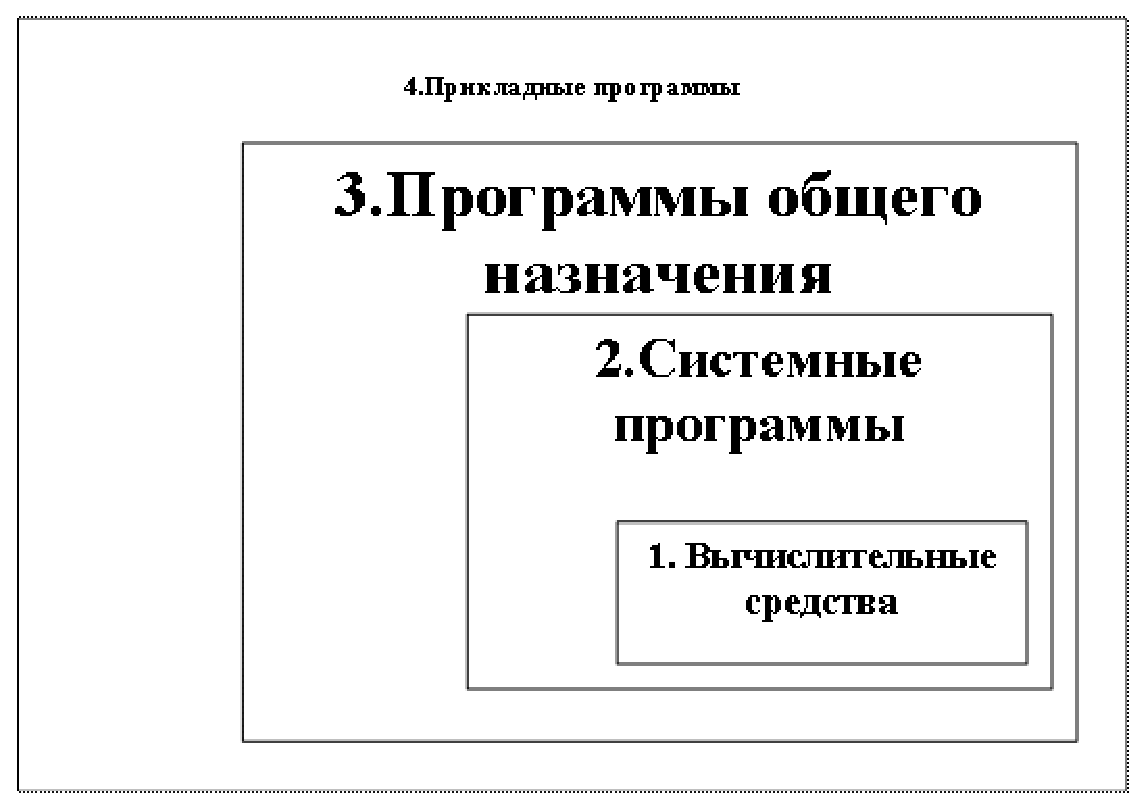
\includegraphics[width=0.6\linewidth]{pon1}}
\caption{Многоуровневый программно-вычислительный комплекс}
\label{mnogour_pvk:pon1}
\end{figure}

В свете всего сказанного предлагается следующая этапность оценки:

1-й этап – осуществляется оценка выполнения требований к качеству комплекса на первом уровне. Здесь исследуются и оцениваются характеристики преимущественно технических средств с использованием широкой номенклатуры специальных или специализированных тестов.

2-й этап – осуществляется оценка уже программно – аппаратного комплекса, включающего средства 1-го и 2-го уровней (технические средства и системные программные средства). При исследованиях и оценках используются имитаторы (в том числе программные) сигналов внешних устройств и функционирования программ общего назначения.

3-й этап – осуществляется оценка программно – аппаратного комплекса, включающего средства 1-го, 2-го и 3-го уровней (технические средства, системные программные средства и программные средства общего назначения). При оценках также используются независимые имитаторы сигналов внешних устройств, функционирования программ общего назначения и прикладных программ.

И, наконец, на 4-м этапе осуществляется оценка характеристик качества всего программно-вычислительного комплекса в целом. При этом используются результаты всех предыдущих этапов, что повышает достоверность и доверие к полученным оценкам.

Обязательные требования к продукции (работам и услугам) по действующему законодательству Российской Федерации устанавливаются Техническими регламентами, принимаемыми в качестве Федеральных законов. Сегодня необходимость технического регламента, устанавливающего обязательные требования по информационной безопасности к программно-вычислительным комплексам очевидна. При этом основным инструментом контроля соблюдения таких требований является сертификация (подтверждение соответствия). Место Системы сертификации в рамках проведения единой технической политики России в области решения задач информатизации поясняется рисунком \ref{sistsert:pon2}.

\begin{figure}[h!]
\center{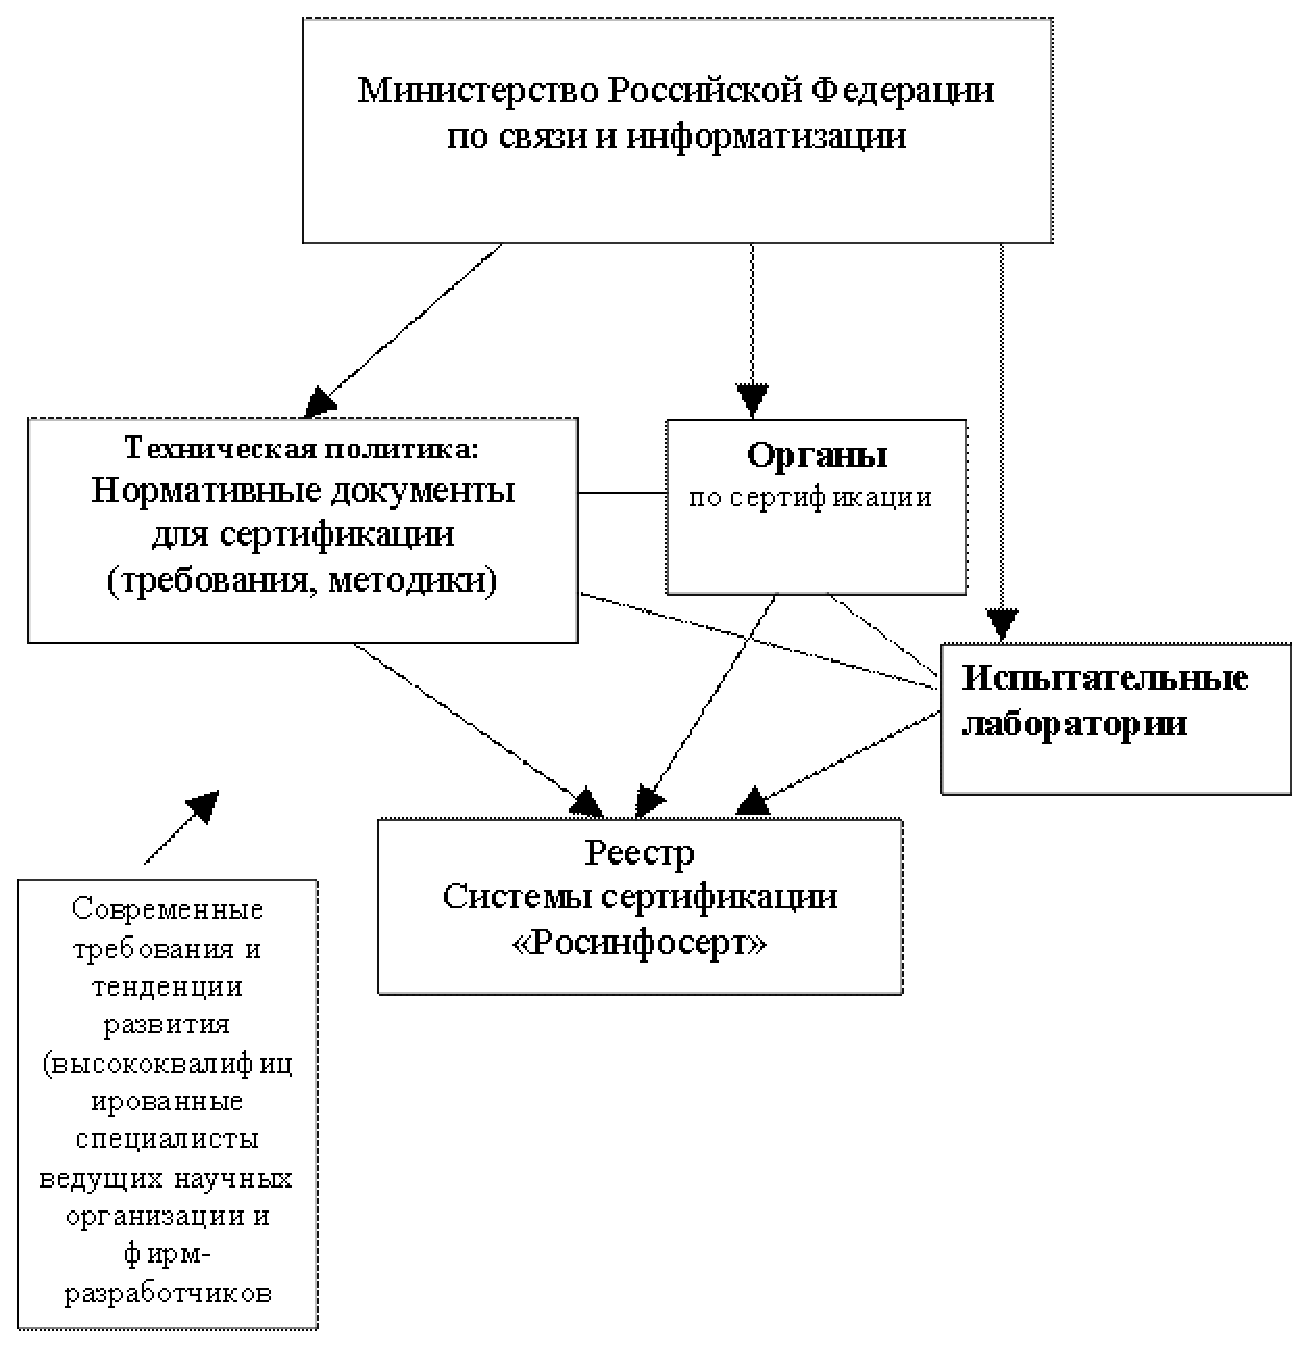
\includegraphics[width=0.8\linewidth]{pon2}}
\caption{Cистема сертификации при проведении единой технической политики}
\label{sistsert:pon2}
\end{figure}

Регистрация в реестре Системы сертифицированной продукции и выдача сертификата соответствия заявителю.
Применение результатов сертификации продукции можно проиллюстрировать примером проведения тендера на поставку средств информатизации для государственных нужд. Схема проведения такого тендера представлена на рисунке \ref{tender:pon3}.

\begin{figure}[h!]
\center{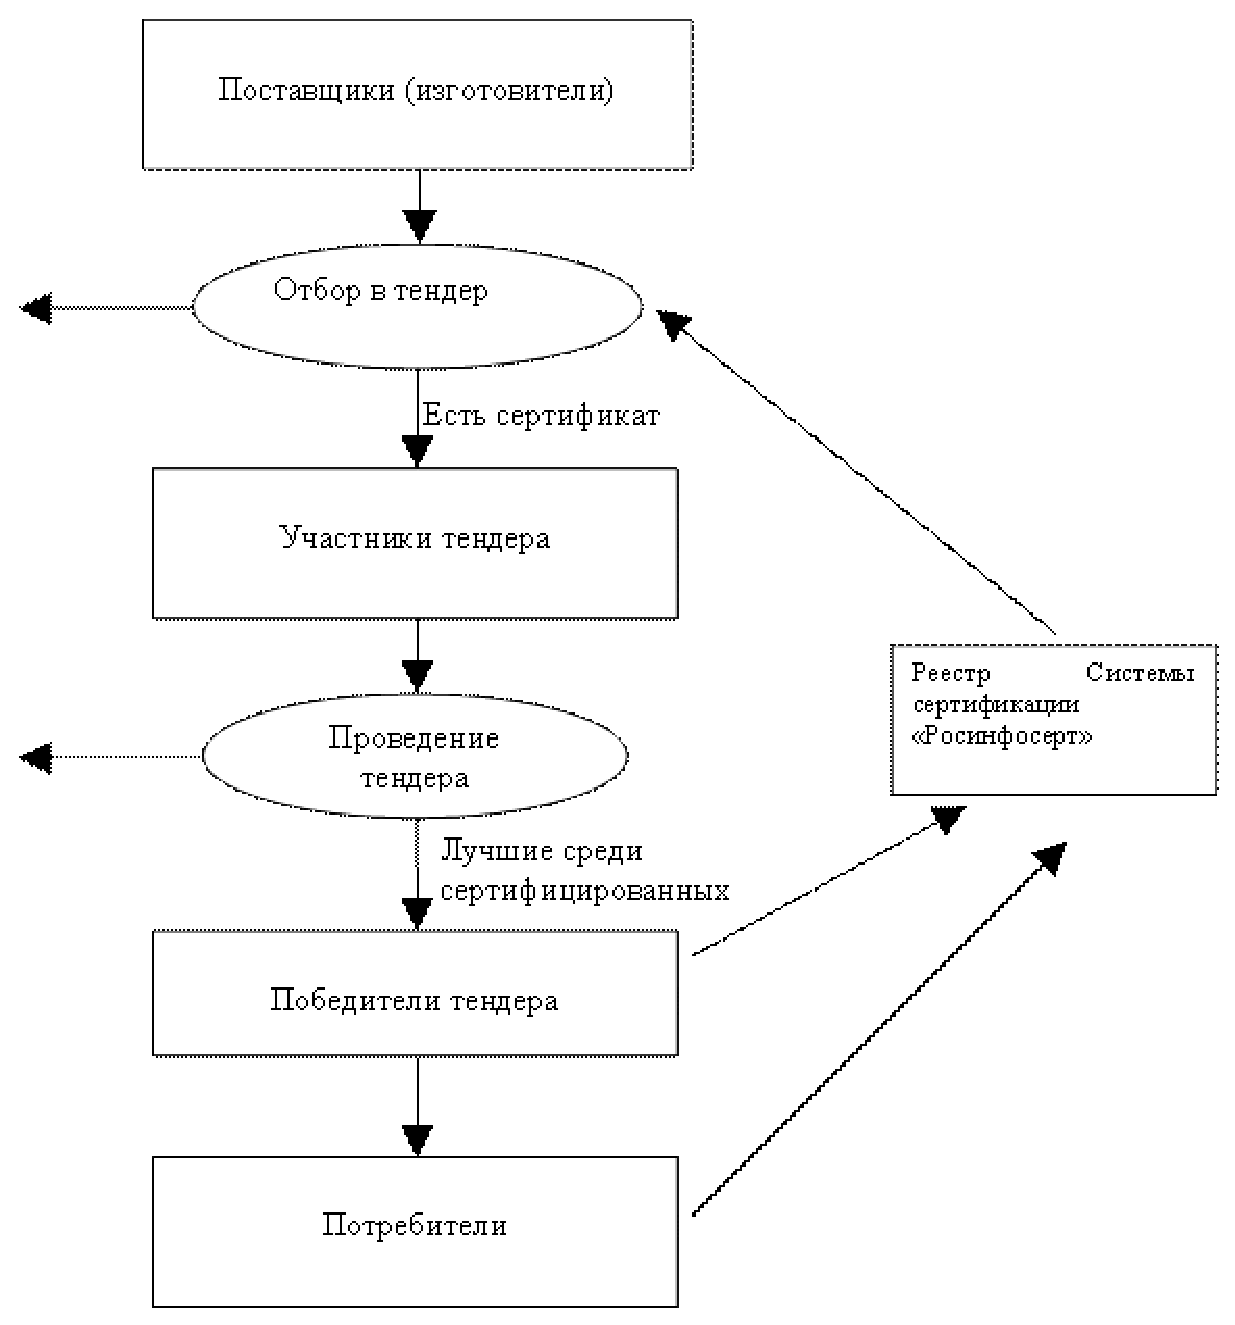
\includegraphics[width=0.8\linewidth]{pon3}}
\caption{Схема проведения тендера на поставку средств информатизации для государственных нужд}
\label{tender:pon3}
\end{figure}

Отбор участников тендера целесообразно проводить на основе анализа результатов их деятельности, одним из объективных показателей которой является сертификат соответствия системы менеджмента качества организации требованиям международных стандартов ИСО 9001 – 2001, а также наличие в номенклатуре выпускаемой продукции сертифицированных продуктов, характеристики которых представлены в Реестре Системы. Такой подход ставит барьер недобросовестным поставщикам и некачественной продукции на рынок средств информатизации России.

В этом случае нормативно-правовое обеспечение применения сертификации для реализации обязательных требований информационной безопасности составляют следующие документы:

\begin{enumerate}
\item Соглашение о взаимодействии в области сертификации средств информатизации между Минсвязи России и субъектом равного уровня. Такое соглашение является необязательным, но желательным документом, который регламентирует взаимоотношения руководства Системы сертификации, ее органов и испытательных лабораторий с потенциальными поставщиками и потребителями средств информатизации, впрямую не подчиняющимися Минсвязи России.
\item Распоряжение (постановление, приказ) субъекта об утверждении Положения о порядке использования средств информатизации для решения своих задач.
\item Положение о порядке использования субъектом средств информатизации, устанавливающее систему показателей и правил отбора и применения поставляемых для государственных нужд средств информатизации.
\item Нормативный документ для сертификации, содержащий состав характеристик средства информатизации, их допустимые значения и способы оценки. Этот документ носит статус стандарта организации, утверждается Минсвязи России по согласованию с субъектом.
\end{enumerate}


\section{Создание собственного репозитория для debian и ubuntu}
\setcounter{figure}{0}
С развитием разрабатываемого программного комплекса возникла необходимость организовать свой репозиторий. Свой репозиторий нужен для того, чтобы выложить программное обеспечение в открытый доступ в удобном для установки и обновления виде.

\subsection{Порядок конфигурирования репозитория}

Для начала следует выбрать дирректорию, в которой мы хотим выкладывать наши deb пакеты. Пускай это будет /var/www/repositories/debian.

\begin{lstlisting} 
prefix=/var/www/repositories/debian
mkdir -p \$prefix/main 
\end{lstlisting}

Копируем все необходимые deb пакеты в /var/www/repositories/debian/main, там можно устроить любую структуру каталогов. Сделаем подкаталоги для каждого пакета и положим в них файлы .deb, .dsc, .changes и .tar.gz. Далее переходим в корень нашего репозитория.

\begin{lstlisting}
cd \$prefix 
\end{lstlisting}

Создаем индексные файлы. Для бинарных пакетов сделать это можно с помощью команды dpkg-scanpackages.

\begin{lstlisting}
dir=\$prefix/dists/unstable/main/binary-i386\\
mkdir -p \$dir\\
dpkg-scanpackages --arch i386 main /dev/null > \$dir/Packages\\
gzip -9c <\$dir/Packages >\$dir/Packages.gz\\
bzip2 -9c <\$dir/Packages >\$dir/Packages.bz2
\end{lstlisting}

Проделаем это для каждой архитектуры, для которой есть пакеты в main. Затем необходимо создать индексные файлы для исходных текстов

\begin{lstlisting}
dir=\$prefix/dists/unstable/main/source\\
mkdir -p \$dir\\
dpkg-scansources main /dev/null > \$dir/Sources\\
gzip -9c <\$dir/Sources >\$dir/Sources.gz\\
bzip2 -9c <\$dir/Sources >\$dir/Sources.bz2
\end{lstlisting}

И наконец, необходимо создать файл \$prefix/dists/unstable/main/Release, который имеет следующую структуру:

\begin{lstlisting}
Archive: unstable
Suite: unstable
Component: main
Origin: название моей организации
Label: Debian репозиторий моей организации
Architecture: архитектуры
\end{lstlisting}

Создадим такой файл и заполним необходимые поля, затем дадим команды

\begin{lstlisting}
dir=\$prefix/dists/unstable/main
apt-ftparchive release \$dir >>\$dir/Release
\end{lstlisting}

Последняя команда вычисляет MD5Sum, SHA1 и SHA256 для файлов Packages* и Sources*.

Теперь осталось только подписать репозиторий. Сделаем это следующей командой:

\begin{lstlisting}
gpg -abs -o \$dir/Release.gpg \$dir/Release
\end{lstlisting}

Для того, чтобы aptitude, apt и др. смогли найти новый репозиторий, добавим необходимые записи в /etc/apt/sources.list.

\begin{lstlisting}
deb http://example.com/repository/debian unstable main
deb-src http://example.com/repository/debian unstable main
\end{lstlisting}


\newpage
\section{Цели следующего семестра}
\begin{enumerate}
\item тестирование системы;
\item подготовка deb-пакета, лицензии;
\item написание публикации.
\end{enumerate}


\section{Заключение}
В данном семестре нашей группой была выполнена часть работы по созданию автоматизированного программного комплекса для проведения компьютерной экспертизы, проанализированы дальнейшие перспективы и поставлены цели на следующий семестр.

\newpage
\renewcommand{\refname}{Список использованных источников}
\bibliography{biblio/lit}

\ESKDappendix{Обязательное}{\normalfont Компакт-диск}
Компакт-диск содержит: 
\begin{itemize}
\item электронную версию пояснительной записки в форматах *.tex и *.pdf;
\item актуальную версию программного комплекса для проведения компьютерной экспертизы;
\item тестовые данные для работы с программным комплексом.
\end{itemize}

\end{document}
